\documentclass{beamer}
\usepackage{graphicx} % Required for inserting images
\usepackage[utf8]{inputenc}
\usepackage{mathtext}
\usepackage[T2A]{fontenc}
\usepackage[english, russian]{babel}
\usepackage{epigraph}
\usepackage{multirow}
\usepackage{amsmath, amsfonts, amssymb}
\usepackage{graphicx}
\usepackage{tikz}
\usepackage{pgfplots}
\usepackage{adjustbox}
\graphicspath{Images}
\pgfplotsset{width=10cm,height=7cm,compat=newest}


\usetheme{Antibes}
\useinnertheme{rectangles}
\useoutertheme{infolines}
\usecolortheme{spruce}
\usecolortheme{dolphin}
\usecolortheme{lily}
\usefonttheme{structurebold}

\title{Непараметричесие критерии\\
статитистическго анализа}
\author{Эрнест Александров ПМИб-3301-52-00}
\date{}
\institute{ВятГУ, 2024}

\begin{document}
\selectlanguage{russian}

\begin{frame}
    \titlepage
\end{frame}

\begin{frame}{}
    \tableofcontents[currentsections]
\end{frame}

\section{Общие определения}
\begin{frame}{Общие определения}
    \textbf{\textit{Статистические гипотезы}} – это предположения или допущения о неизвестных параметрах, выражаемых в терминах вероятности, которые могут быть проверены на основании выборочных показателей с помощью статистических критериев.
    
    \begin{columns}
        \pause
        \column{.5\textwidth}
            \begin{block}{Параметрические методы}
            \textbf{Требуют} обязательного знания закона распределения изучаемых признаков в совокупности и вычисления их основных параметров
            \end{block}
        \pause
        \column{.5\textwidth}
            \begin{block}{Непараметрические методы}
            \textbf{Не требуют} знания закона распределения изучаемых признаков в совокупности и вычисления их основных параметров
            \end{block}       
    \end{columns}
\end{frame}

\begin{frame}{Общие определения}
    \textbf{\textit{Статистический критерий (К)}} (критерий значимости) – это некий параметр, вычисленный по определенному алгоритму, который используется для проверки основной гипотезы.
    
    \begin{columns}
        \pause      
        \column{.5\textwidth}
        \begin{block}{Параметрические критерии:}
            \begin{enumerate}[<+->]
                \item критерий Стьюдента;
                \item критерий Фишера,
                \item критерий Романовского.
            \end{enumerate}
        \end{block} 
        \pause
        
        \column{.5\textwidth}
        \begin{block}{Непараметрические критерии:}
            \begin{enumerate}[<+->]
                \item критерий знаков;
                \item критерий Пирсена;
                \item критерий Манна-Уитни.
            \end{enumerate}
        \end{block}      
    \end{columns} 
\end{frame}

\section{Критерий знаков}
\subsection{История}
\begin{frame}{Критерий знаков (G-критерий)}{История}
    \begin{columns}
        \column{.5\textwidth}
            \begin{block}{}
            Данный критерий был разработан доктором \textbf{Джоном Арбетнотом} – шотландским врачом, сатириком и эрудитом в 1710 году. Критерий предназначен для сравнения состояния некоторого свойства у членов двух \textbf{зависимых выборок} на основе измерений.
            \end{block}
        \column{.5\textwidth}
                \begin{figure}[htbp]
                    \label{fig:john-arbuthnot}
                    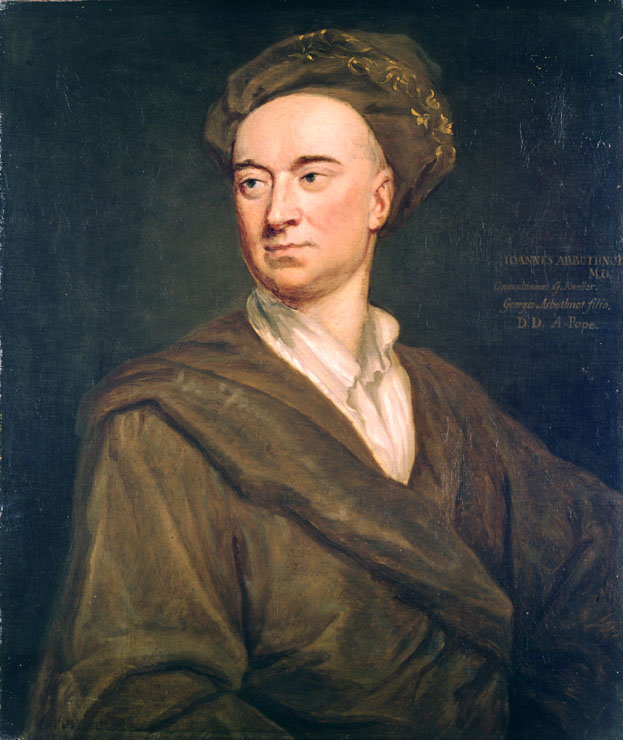
\includegraphics[height=120pt]{Images/Arbuthnot_John_Kneller.jpg}
                \end{figure}
    \end{columns}
\end{frame}

\subsection{Принцип работы}
\begin{frame}{Критерий знаков (G-критерий)}{Принцип работы}
        Имеется две серии наблюдений над случайными переменными $X$ и $Y$, полученные при рассмотрении двух {\textbf{зависимых выборок}}. На их основе составлено N пар вида $(x_i, y_i)$, где $x_i, y_i$ – результаты двукратного измерения одного и того же свойства у одного и того же объекта.

        \smallskip
        Элементы каждой пары $x_i, y_i$ сравниваются между собой по величине, и паре присваивается знак «+», если $x_i < y_i$ , знак «–», если $x_i > y_i$  и «0», если $x_i = y_i$.

        \pause
        \smallskip
        \textbf{\textit{Нулевая гипотеза}} формулируются следующим образом: в состоянии изучаемого свойства нет значимых различий при первичном и вторичном измерениях.

        \pause
        \smallskip
        \textbf{\textit{Альтернативная гипотеза}}: законы распределения величин $X$ и $Y$ существенно различны в одной и той же совокупности при первичном и вторичном измерениях свойства.
\end{frame}

\section{Критерий Пирсона}
\subsection{История}
\begin{frame}{Критерий Пирсона (хи-квадрат)}{История}
    \begin{columns}
        \column{.5\textwidth}
            \begin{figure}[htbp]
                \label{fgr:karl-pearson}
                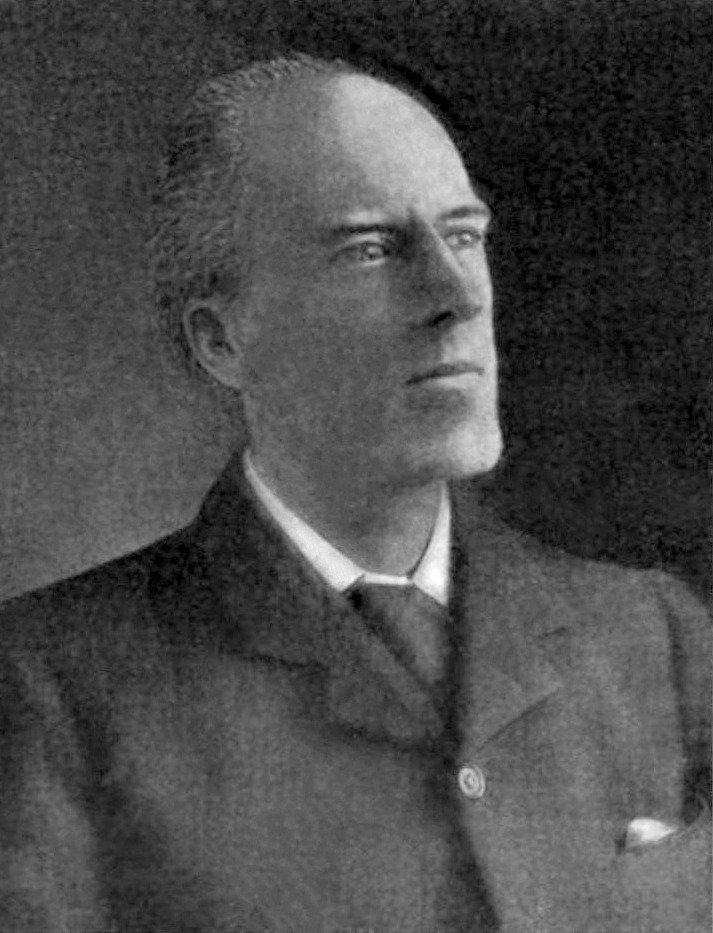
\includegraphics[height=130pt]{Images/karl-pearson.jpg}
            \end{figure}
        \column{.5\textwidth}
            \begin{block}{}
                Предложенный в 1900 году английским математиком \textbf{Карлом Пирсоном} критерий согласия $\chi^2$ (хи-квадрат) применяется для сравнения распределений объектов двух совокупностей на основе измерений по шкале наименований в двух \textbf{независимых выборках}
            \end{block}
    \end{columns}
\end{frame}

\subsection{Принцип работы}
\begin{frame}{Критерий Пирсона (хи-квадрат)}{Принцип работы}
    \small
    Предположим, что состояние изучаемого свойства (например, выполнение определенного задания) измеряется у каждого объекта по шкале наименований, имеющей только две взаимоисключающие категории (например, верно – неверно). По результатам измерения состояния изучаемого свойства у объектов двух выборок составляется четырехклеточная таблица

    
    \begin{table}[h]
        \label{tbl:measurement-results}
        \centering
        \begin{tabular}{c|c|c|c} 
             &\textbf{Категория1}&\textbf{Категория2}&  \\
             \cline{2-3} \textbf{Выборка № 1}&\textit{$O_{11}$}&\textit{$O_{12}$}&\textit{$O_{11} + O_{12} = n_1$} \\
             \cline{2-3}\textbf{Выборка № 2}&\textit{$O_{21}$}&\textit{$O_{22}$}&\textit{$O_{21} + O_{22} = n_2$} \\
             \cline{2-3}&\textit{$O_{11} + O_{21}$}&\textit{$O_{21} + O_{22}$}&\textit{$n_1 + n_2 = N$}  \\
        \end{tabular}
    \end{table}
        
    В этой таблице $О_{ij}$ – число объектов в $i-ой$ выборке, попавших в $j-ую$ категорию по состоянию изучаемого свойства; $i=1,2$ – число выборок; $j=1,2$ – число категорий; $N$ – общее число наблюдений, равное  $n_1+n_2$
\end{frame}

\begin{frame}{Критерий Пирсона (хи-квадрат)}{Принцип работы}
    Тогда на основе данных таблицы можно проверить нулевую гипотезу о равенстве вероятностей попадания объектов первой и второй совокупностей в первую (вторую) категорию шкалы измерения проверяемого свойства

    \pause
    \smallskip
    Для проверки рассмотренных выше нулевых гипотез по данным таблицы подсчитывается значение статистики критерия $Т_{эмп}$ по следующей формуле:

    $$
        T=\frac{N\cdot (|O_{11} \cdot O_{22} -O_{12} \cdot O_{21}| - \frac{N}{2})^2}{n_1 \cdot n_2 \cdot (O_{11} + O_{21}) \cdot (O_{12} + O_{22})}
    $$

    где $n_1, n_2$ – объемы выборок, $N$ – общее число наблюдений
\end{frame}

\section{U-критерий Манна-Уитни}
\subsection{История}
\begin{frame}{U-критерий Манна – Уитни}{История}
    Этот метод сравнения двух выборок признается наиболее чувствительным и мощным среди прочих непараметрических критериев. Он был предложен в 1945 году \textbf{\textit{Фрэнком Уилкоксоном}}. В 1947 году он был существенно переработан и расширен \textbf{\textit{Х.Б.Манном}} и \textbf{\textit{Д.Р.Уитни}}, по именам которых и называется.

    \begin{figure}[h]
        \centering
        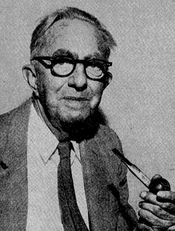
\includegraphics[height=100pt]{Images/FrankWilcoxon.png}
        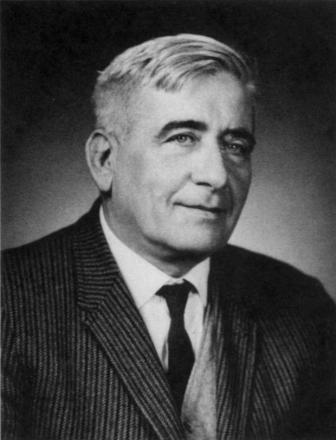
\includegraphics[height=100pt]{Images/mann.jpg}
        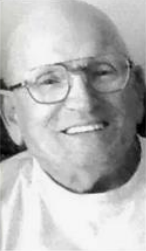
\includegraphics[height=100pt]{Images/Whitney.png} \\
        \scriptsize
        Ф.~Уилкоксон, Х.~Б.~Мани и Д.~Р.~Уитни (слева направо)
    \end{figure}
\end{frame}

\subsection{Принцип работы}
\begin{frame}{U-критерий Манна – Уитни}{Принцип работы}
    \footnotesize
    Согласно нулевой гипотезе, сравниваемые совокупности имеют одинаковые распределения. Техника метода состоит в том, что все варианты сравниваемых совокупностей ранжируют в одном общем ряду: каждому значению присваивают ранг, порядковый номер. При этом одинаковым (повторяющимся) значениям вариант должен соответствовать один и тот же средний ранг (они как бы «делят места»). После этого ранги вариант суммируют отдельно по каждой выборке и вычисляют величину критерия:
    \begin{columns}
        \pause
        \column{.25\textwidth}
        $$
            R_1=\sum_{i=1}^{n_1} r_i
        $$
        \pause
        \column{.25\textwidth}
        $$
            R_1=\sum_{i=1}^{n_1} r_i
        $$
        \pause
        \column{.50\textwidth}
        $$
            T =\frac{U - 0.5 \cdot n_1 \cdot n_2}{\sqrt{(n_1 \cdot n_2 \cdot (n+1)/12)}}
        $$      
    \end{columns}

    \smallskip
    \pause
    где $U = max(U_1, U_2)$ – максимальное значение из двух величин:
    \begin{columns}
        \column{.50\textwidth}
        $$
            U_1 = n_1 \cdot n_2 + 0.5 \cdot n_1(n_1+1)-R_1
        $$
        \column{.50\textwidth}
        $$
            U_2 = n_1 \cdot n_2 + 0.5 \cdot n_2(n_2+1)-R_2
        $$      
    \end{columns}

    \pause
    \medskip                          
    Если выборка достаточно велика ($n > 20$), величина статистики $Т_{эмп}$ сравнивается с табличным значением критерия Стьюдента для $df = \infty$ и $\alpha = 0.1$.
\end{frame}

\section{Заключение}
\begin{frame}{Заключение}
    В данной работе были рассмотрены три непараметрических критерия методов математической статистики: критерий знаков, критерий Пирсона (хи-квадрат) и U-критерий Манна – Уитни.

    \pause
    \smallskip
    Следует, однако, отметить, что список непараметрических критериев не ограничивается указанными. Выделяют также следующие непараметрические критерии :

    \begin{itemize}[<+->]
        \item Q-критерий Розенбаума;
        \item критерий Колмогорова-Смирнова;
        \item критерий Андерсона-Дарлинга;
        \item критерий согласия Кёйпера
    \end{itemize}
\end{frame}

\section{Introduction}

\end{document}
